The concept behind the implementation was to make a highly object oriented framework
so that the different parts could be replaced by new ones transparently and thus allowing
for further experimentation and expansion of the tool.
The chosen language for the implementation was Java, since Java is a popular programming language
it opens up the possibility of using the tool with many other packages or even as a webservice
for more sophisticated applications.

\subsection{Packages}

This is a description of the most important  packages and classes related to the implementation:


\subsubsection*{IO}
The classes in this package have the responsability of dealing with
the input/output files.\\
The class DictionaryReader.java is incharged of reading a raw dictionary file (one entry per line).

\subsubsection*{Measures}
This package is composed of all classes relating the different similarity measures.
The SimString algorithm is independant of the chosen similarity, for doing this
an interface called $Similarity$ exists within the package, in order to extend
the system to provide new similarities measures this interface has to be implemented.\\
\\
Aditionally this package has a class name MeasureFactory, which is incharged of constructing
similarities's objects.

\begin{figure}[h!]
  \caption{Class Diagram with respect to Similarity classes}
  \centering
    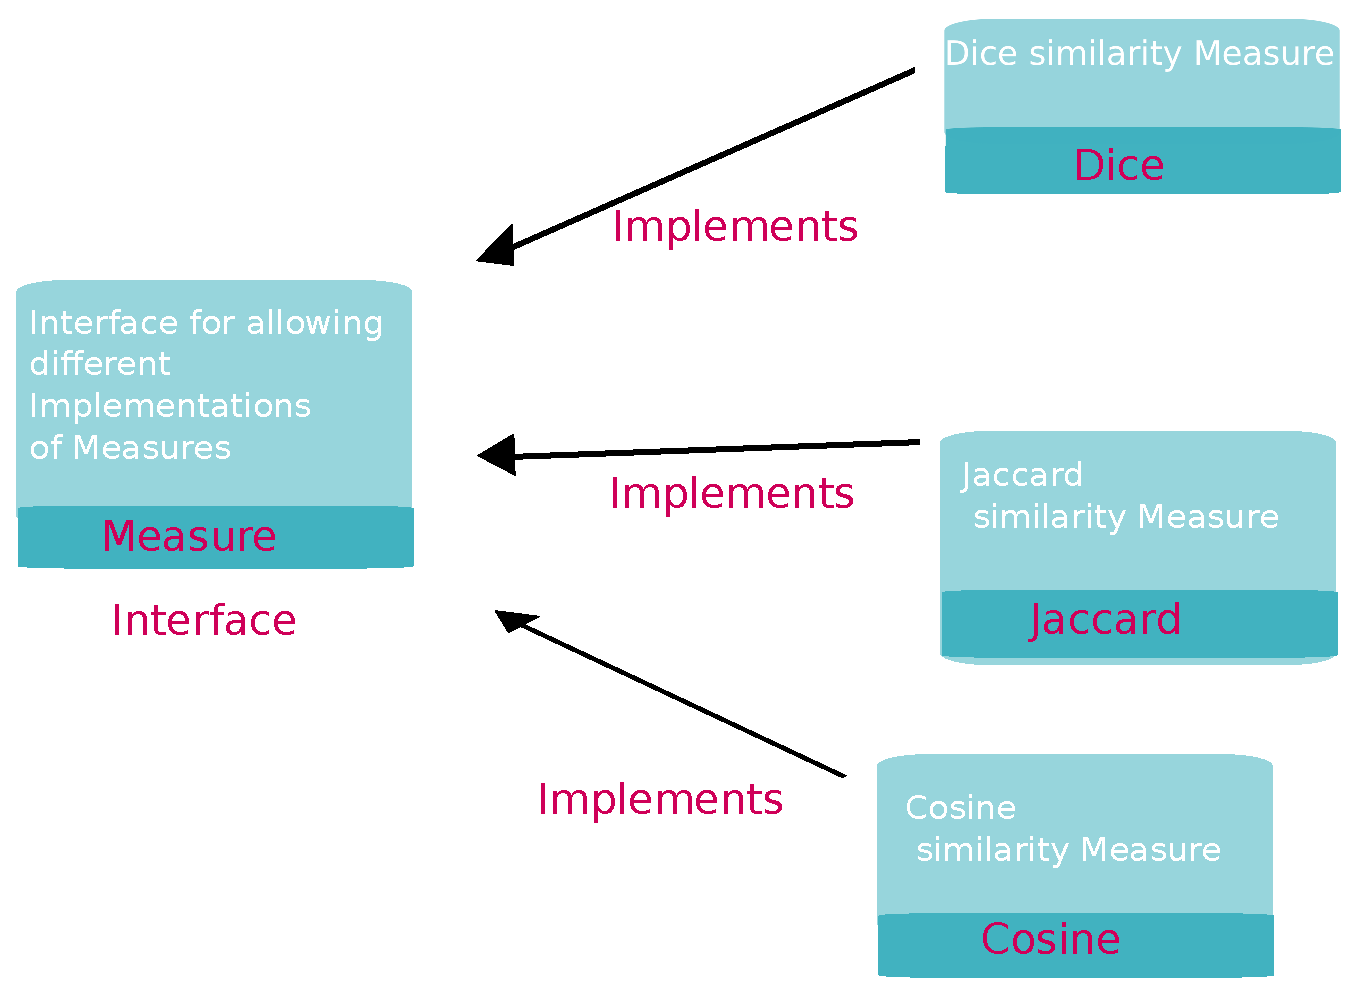
\includegraphics[scale=0.45]{graphics/similarities}
   \label{fig:similarityClasses}  
\end{figure}


\subsubsection*{Dictionary}
This package contains all the classes which have a responsability related to dictionaries.\\
\\
Among the most important ones are $LowLevelDictionaryImplementation$ this is an interface
which allows the tool to implement differnt kinds of Dictionary Implementations, for example
one dictionary can be represented either as a hashtable or as suffixtree, while those
data structures are different by implementing $LowLevelDictionaryImplementation$ they become
transparent to the simString algorithm.\\
\\
Additionally this package contains all the classes related to the different offered implementations
of dictionaries.




\subsubsection*{SimString}
This package contains the class $SimString$ which given a dictionary,a similarity configuration  and a query
is able to search in the dictionary and retrieve all the similar NE given the value of the parameters.


\subsubsection*{Util}
This package is composed of different classes with different responsabilities.
The $NGram$ class is incharged of splitting words into ngrams and dealing with any specific functionality related to ngrams.

\subsubsection*{Examples}
This package contains classes (each one is an example) for the potential users.

\subsubsection*{Test}
This package contains classes which allow team to asses the time performance of the tool and make comparisons among the different implementations.


\subsection{Dictionary Implementations}


As an addition to the simstring algorithm, the team introduced different ways to implement
the underlying data structure representing the ngram-inverted index.\\
\\
There are two types of data structures alternatives: mapped and not mapped.
Not mapped data structures are traditional data structures, that is, structures that are kept entirely on memory while the program is running. \\
As opposed to this type  there are mapped data structures which are data structures saved in the hard disk
and as data from it is needed small chunks of the datastructure are loaded into memory.\\
\\
The memory mapped data structures are ideally for cases when the number of data being stored is very high and having the whole datastructure in memory at once is not feasible.
However memory mapped data structures come with a cost: $Memory$.\\
Since memory mapped data structure implementations want to be as fast as traditional data structures, they have to be stored in memory in a way they can be queried quickly.\\
The only way to assure this is by having a fixed number of bits used per data field in the mapped data structure,this means, that no matter the size of the data, a slot in this structures will always have a fix size, this means using extra memory.


\begin{figure}[h!]
  \caption{The Dictionary Implementations}
  \centering
    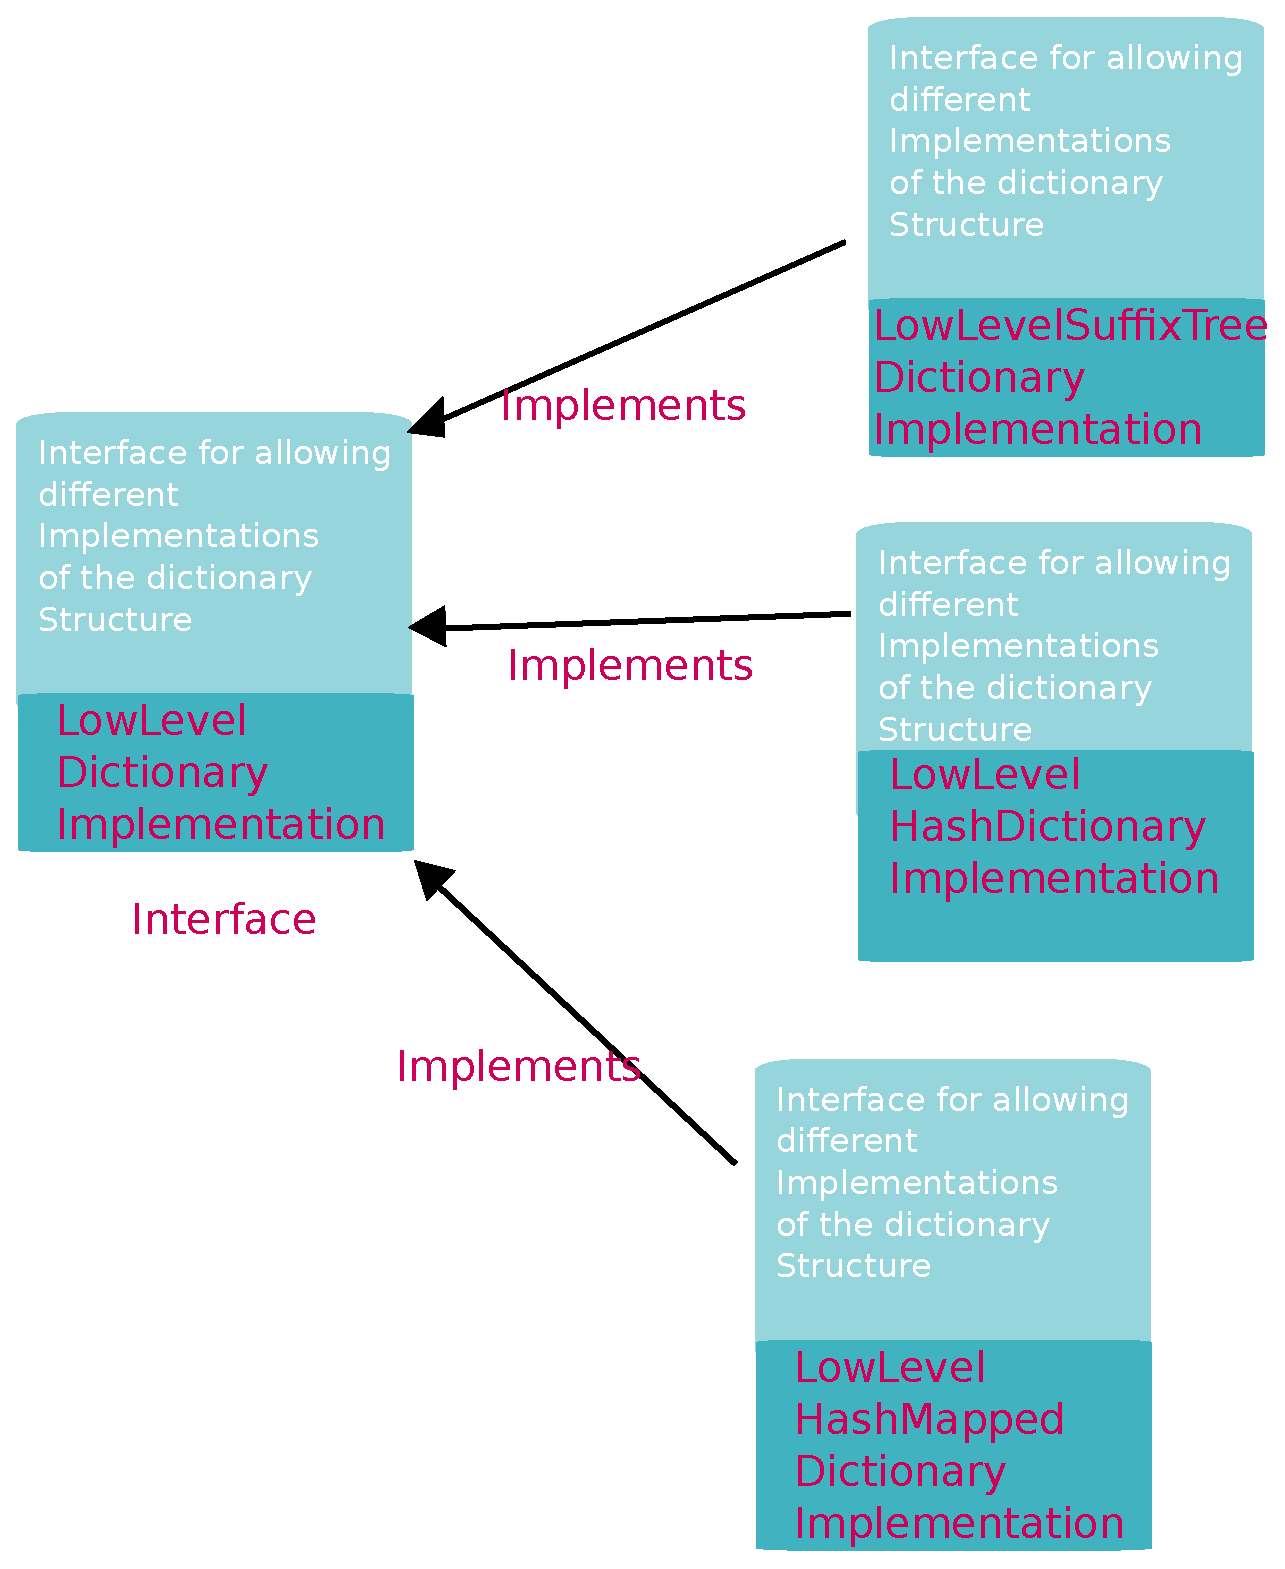
\includegraphics[scale=0.45]{graphics/dictionaryImplementations}
   \label{fig:dictionaryClasses}  
\end{figure}



\subsubsection{SuffixTree}  

This is an implementation of the inverted index of ngrams by using suffixTrees.\\
The keys in this case are strings of the shape: $ngram$-$sizeOfString$, the values are Priority Queues with the id's of dictionary entries which size is $sizeOfString$ and contains the given  $ngram$.

\subsubsection{Naive-HashTable}
 This is an implementation of the inverted index of ngrams by using Java HashMaps.\\
The keys in this case are strings of the shape: $ngram$-$sizeOfString$, the values are Priority Queues with the id's of dictionary entries which size is $sizeOfString$ and contains the given  $ngram$.
  
\subsubsection{MemoryMapped Hashtable}
 This is an implementation of the inverted index of ngrams by using memory mapped Hashtables.\\
It allows to save the generated dictionary in a file and to load it for later use.

\begin{figure}[h!]
  \caption{Comparison between Mapped Datastructures and not mapped}
  \centering
    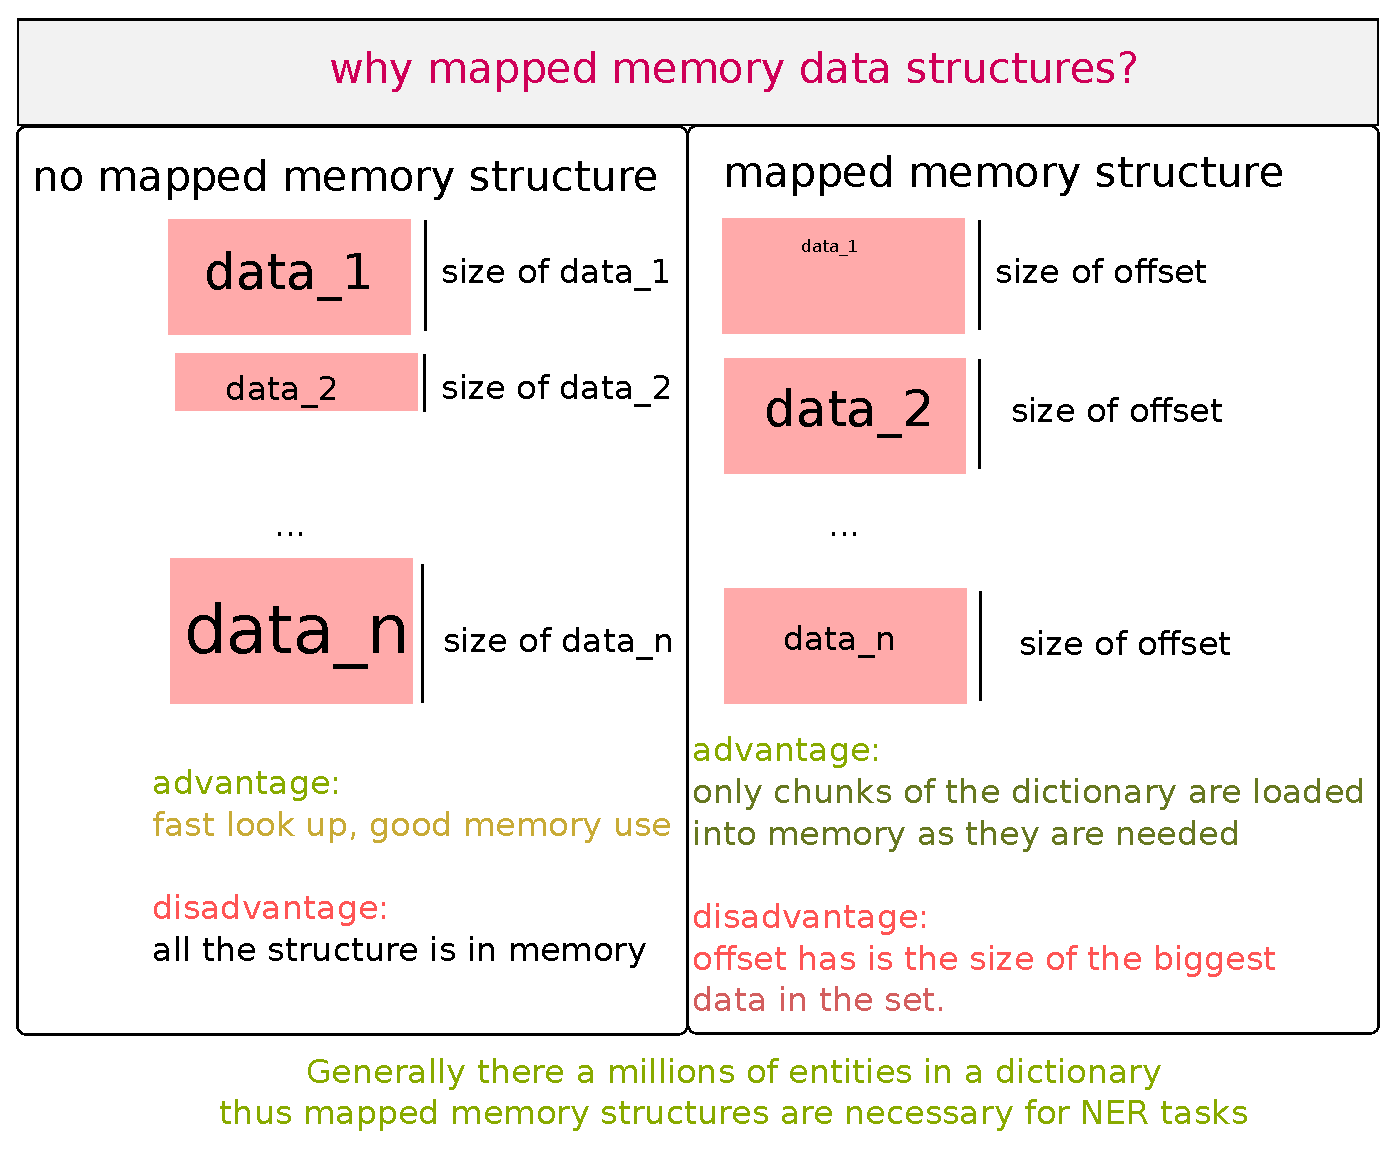
\includegraphics[scale=0.5]{graphics/memoryMappedVsNonMemoryMapped}
   \label{fig:mappedDataStructures}  
\end{figure}


  
